\section{Integration over lines, surfaces, and volumns}
\subsection{Line integrals}
\begin{definition}
    For vector field $ \mathbf{F} = \mathbf{F}(\mathbf{x}) $ and \textit{piecewise smooth} parametrised curve $ C= [a,b]\ni t \mapsto \mathbf{x}(t) $, we define the \textbf{line integral}
    \[
        \int_{C} \mathbf{F} \cdot\mathrm{d}\mathbf{x} = \int_{a}^{b} \mathbf{F}(\mathbf{x}(t)) \cdot \frac{\mathrm{d}\bfx}{\mathrm{d}t}\dd t. 
    \]
    If we want to integrate in opposite direction, write 
    \[
        \int_{-C} \mathbf{F} \cdot\mathrm{d}\mathbf{x}.
    \]
\end{definition}
\begin{note}
    We can intepret it as the work done by a particle moving along $C$ in presence of a force $ \mathbf{F}. $
\end{note}

Note that
\[
    \int_{C} F \cdot\mathrm{d}\mathbf{x} \approx \sum_{i} \mathbf{F}(\bfx_i) \cdot \Delta \bfx_i,
\]
where $ \Delta\bfx_i = \bfx_{i+1}-\bfx_{i} $.

\begin{center}
    \begin{tikzpicture}[scale=0.7]
        \node [dot] (0) at (-4, -2) {};
        \node [below] at (0) {$ \bfx_0 $};
        \node [dot] (1) at (5, 3) {};
        \node [right] at (1) {$ \cdots $};
        \node [dot] (2) at (-2, 2) {};
        \node [above] at (2) {$ \bfx_1 $};
        \node (3) at (1, -1) {};
        \node [dot] (4) at (-0.55, 0.5) {};
        \node [below left] at (4) {$ \bfx_2 $};
        \node [dot] (5) at (2.225, 0) {};
        \node [below right] at (5) {$ \bfx_3 $};
        \draw [in=-165, out=75, looseness=0.75] (0) to (2.center);
        \draw [in=-165, out=0, looseness=0.75] (2.center) to (3.center);
        \draw [in=-180, out=15, looseness=0.75] (3.center) to (1);
        \draw [->-=0.5,blue] (0) to (2.center);
        \draw [->-=0.5,blue] (2.center) to (4.center);
        \draw [->-=0.5,blue] (4.center) to (5.center);
        \draw [->-=0.5,blue] (5.center) to (1);
    \end{tikzpicture}
\end{center}

\begin{example}\label{eg:3.1}
    Consider $ \mathbf{F} = (x^2y,yz,2zx) $ and consider two curves connecting origin to $ (1,1,1) $:
    \[
        C_1: [0,1]\ni t \mapsto \begin{pmatrix}
            t \\ t \\ t
        \end{pmatrix},\quad 
        C_2 : [0,1]\ni \mapsto \begin{pmatrix}
            t \\ t \\ t^2
        \end{pmatrix},
    \]
    so 
    \[
        \int_{C_1} \mathbf{F} \cdot\mathrm{d}\mathbf{x} = \int_{0}^{1} \begin{pmatrix}
            t^3 \\ t^2 \\ 2t^2
        \end{pmatrix}\cdot \begin{pmatrix}
            1 \\ 1 \\ 1
        \end{pmatrix} \,\mathrm{d}t = \frac{5}{4},
    \]
    and 
    \[
        \int_{C_2} \bfF \cdot\mathrm{d}\mathbf{r} = \int_{0}^{1} \begin{pmatrix}
            t^3 \\ t^3 \\ 2t^3
        \end{pmatrix}\cdot \begin{pmatrix}
            1 \\ 1 \\ 2t
        \end{pmatrix} \,\mathrm{d}t = \frac{13}{10}.
    \]
    We see that in general, line integrals between 2 points depend on paths taken.
\end{example}
\begin{example}
    A particle at $ \bfx $ experiences force in cylindrical polars by
    \[
        \mathbf{F}(\mathbf{x}) = z\rho\bfe_\phi.
    \]
    Calculate the work done by travelling along the path
    \[
        C: [0,2\pi]\ni t \mapsto \begin{pmatrix}
            a\cos t \\ a\sin t \\ t
        \end{pmatrix}(a>0).
    \]
    Recall the line element in cylindrical polars
    \[
        \rmd \mathbf{x} = \rmd \rho\,\bfe_\rho+\rho\dd \phi\,\bfe_\phi+\rmd z\,\bfe_z,
    \]
    so $ \mathbf{F}\cdot \rmd \mathbf{x} = z\rho^2 \dd  \phi $. Also on the path, $ (\rho,\phi,z) = (a,t,t) $, so $ (\rmd \rho,\rmd \phi,\rmd z) = (0,\rmd t,\rmd t) $, and thus $ \mathbf{F}\cdot \rmd \bfx = a^2t\dd t $. Hence
    \[
        \int_{C} \mathbf{F} \cdot\mathrm{d}\mathbf{x} = a^2 \int_{0}^{2\pi} t \,\mathrm{d}t = 2\pi^2 a^2.
    \]
\end{example}

A curve may be \textbf{closed}. That is $ \bfx(a)=\bfx(b) $. In this case we write 
\[
    \oint_{C}\bfF\cdot \rmd\bfx.
\]
We call this kind of integral the \textbf{circulation} of $\bfF$ about $C$.

\begin{example}
    Take exmaple \ref{eg:3.1} with $ C=C_1-C_2 $.
    \begin{center}
        \begin{tikzpicture}
          \node [dot] {};
          \node [left] {$O$};
          \node at (2, 2) [dot] {};
          \node at (2, 2) [right] {$(1,1,1)$};
          \draw [-<-=0.4] (0, 0) parabola (2, 2);
          \node at (1.8, 1) {$C_2$};
          \draw [-<-=0.4] (2, 2) -- (0, 0) node [pos = 0.5, anchor = south east] {$C_1$};;
        \end{tikzpicture}
      \end{center}
      Then 
      \[
          \oint_{C} \bfF \cdot\mathrm{d}\mathbf{x} = \int_{C_1} \bfF \cdot\mathrm{d}\mathbf{x}-\int_{C_2} \bfF \cdot\mathrm{d}\mathbf{x} = -\frac{2}{15}.
      \]
\end{example}

\subsection{Conservative forces and exact differentials}
We have seen how to interpret $ \bfF\cdot\rmd\bfx $. This is another example of \textbf{differential form}.
\begin{definition}[Exact differential, conservative fields]
    We say $\bfF\cdot\rmd\bfx$ is \textbf{exact} if 
    \[
        \bfF\cdot\rmd\bfx = \rmd f
    \]
    for some scalar function $f$. Recall that $ \rmd f = \nabla f\cdot\rmd\bfx $. So $ \bfF\cdot\rmd\bfx $ is exact if and only if $ \bfF = \nabla f $ for some scalar function $f$. We call such vector fields $\bfF$ \textbf{conservative}.
\end{definition}
So we have 
\[
    \bfF\cdot\rmd\bfx \text{ is exact }\Longleftrightarrow \bfF \text{ is conservative}.
\]

\begin{proposition}
    If $ \theta $ is exact, then 
    \[
        \oint_{C} \theta =0
    \]
    for any \textit{close} curve $C$. Equivalently, if $\bfF$ is conservative, then the circulation of $\bfF$ vanishes.
\end{proposition}
\begin{proof}
    By previous, if $ \theta $ exact then $ \theta=\nabla f \cdot \rmd\bfx $ for some $f$. If $ C: [a,b]\ni t \mapsto \bfx(t) $ is close, then 
    \begin{align*}
        \oint_{C}\theta &= \oint_{C}\nabla f\cdot \bfx = \int_{a}^{b} \nabla f((\bfx(t))) \cdot \frac{\mathrm{d}\bfx}{\mathrm{d}t}  \,\mathrm{d}t \\
       & = \int_{a}^{b} \frac{\mathrm{d}}{\mathrm{d}t}\left( f(\bfx(t)) \right)  = f(\bfx(b))-f(\bfx(a)) = 0
    \end{align*}
    by fundamental theorem of calculus.
\end{proof}
\begin{note}
    Might think e.g. in cylindrical polars, that $f(\rho,\phi,z)=\phi$ is a nice ``function'' on $ \mathbb{R}^{3} $. Note that it is infact multivalued at given position.
\end{note}

\begin{corollary}
    If $\bfF$ is conservative, then line integrals of $\bfF$ are independent of the paths taken.
\end{corollary}
\begin{proof}
    Indeed, if $ C_1,C_2 $ are two such paths, then $ C=C_1-C_2 $ is closed and thus
    \[
        \oint_{C}\bfF\cdot\rmd\bfx = 0 \Longleftrightarrow \int_{C_1} \bfF \cdot\mathrm{d}\mathbf{x} = \int_{C_2} \mathbf{F} \cdot\mathrm{d}\mathbf{x}.
    \]
\end{proof}

\begin{proposition}
    Let $(u_1, u_2, u_3) \equiv (u, v, w)$ be an arbitrary set of OCC and let
    \[
        \mathbf{F} \cdot \rmd\bfx = \theta = A(u, v, w) \dd u + B(u, v, w) \dd v + C(u, v, w) \dd w \equiv \theta_i \dd u_i.
    \]
    A \textit{necessary} condition for $ \theta $ to be exact is
    \begin{equation}\label{eq:3.3}\tag{$\dagger$}
        \frac{\partial \theta_i}{\partial u_j}= \frac{\partial \theta_j}{\partial u_i}\quad \text{for each }i,j.  
    \end{equation}
\end{proposition}
\begin{proof}
    Indeed, if $ \theta $ is exact, then $ \theta=\rmd f $ and 
    \[
        \theta = \frac{\partial f}{\partial u_i}\dd u_i \Longleftrightarrow \theta_i = \frac{\partial f}{\partial u_i}  
    \]
    so 
    \[
        \frac{\partial \theta_i}{\partial u_j}= \frac{\partial^2 f}{\partial u_j u_i} =   \frac{\partial^2 f}{\partial u_i u_j} = \frac{\partial \theta_j}{\partial u_i}.
    \]
\end{proof}
\begin{definition}[Closed differentials]
    If a differential form $ \theta = \theta_i\dd u_i $ obeys (\ref{eq:3.3}), it is said to be \textbf{closed}.
\end{definition}
Hence $ \theta $ exact $ \Rightarrow \theta $ closed. The reverse implication is true if the domain $ \Omega\in \mathbb{R}^{3} $ on which $ \theta $ is defined is \textit{simply connected}\footnote{$ \Omega $ is simply connected if all closed \textit{loops} in $ \theta $ can be continuously shrunk to any \textit{point} inside $ \Omega $ without leaving it. Refer to \href{https://www.mv.helsinki.fi/home/pankka/deRham2013}{this note} for details.}.

\begin{example}
    Let $ \theta=y\dd x-x\dd y $. Note that $ \partial y/\partial y=1\neq -1=\partial (-x)/\partial x   $, so it is \textit{not} exact. 
\end{example}

\begin{example}
    Compute 
    \[
        \oint_C 3x^2y\dd x+x^3\dd y,\quad C:[\alpha_1,\alpha_{100}] \ni t \mapsto \begin{pmatrix}
            \cos \left(\Im\left(\zeta\left(\frac{1}{2}+it\right)\right)\right) \\ \sin \left(\Re\left(\zeta\left(\frac{1}{2}+it\right)\right)\right)  \\ 0
        \end{pmatrix},
    \]
    where $ \alpha_1,\alpha_{100} $ are the 1st and 100th zeros of $ \zeta(\frac{1}{2}+it) $. Note that $ 3x^2y\dd x+x^3\dd y=\rmd(x^3y) $ and $C$ is closed, so it is 0.
\end{example}

\begin{example}
    The work done $ \int_{C} \mathbf{F} \cdot\mathrm{d}\mathbf{x} $, where $ C:[a,b]\ni t\mapsto \bfx(t) $ is 
    \[
        \int_{C} \mathbf{F} \cdot\mathrm{d}\mathbf{x}= m \int_{a}^{b} \ddot{\bfx}\cdot \dot{\bfx} \,\mathrm{d}t = \left[ \frac{1}{2}m |\dot{\bfx}|^2 \right].
    \]
    If $\bfF = -\nabla V$ is conservative, then 
    \[
        \int_{C} \mathbf{F} \cdot\mathrm{d}\mathbf{x} = - \int_{C} \nabla V \cdot\mathrm{d}\mathbf{x} = V(\bfx(a))-V(\bfx(b)).
    \]
    Hence
    \[
        \frac{1}{2}m |\dot{\bfx}(a)|^2+V(\bfx(a))=\frac{1}{2}m |\dot{\bfx}(b)|^2+V(\bfx(b)),
    \]
    i.e. total energy is conserved.
\end{example}

\subsection{Integration in $ \mathbb{R}^{2} $}
\subsubsection{Definition}
We want to integrate over bounded region $ D \subseteq \mathbb{R}^{2} $. To do this, cover $D$ with small disjoint $A_{ij}$ with areas $ \delta A_{ij} $, each contained in a disc of radius $ \epsilon>0 $. Let $ (x_i,y_i) $ be points contained in each $A_{ij}$.
\begin{center}
    \begin{tikzpicture}
      \draw [->] (0, 0) -- (6, 0) node [right] {$x$};
      \draw [->] (0, 0) -- (0, 4) node [above] {$y$};
      \draw (2, 1.6) -- (3.6, 1.6);
      \draw (2, 2) -- (3.6, 2);
      \draw (2, 2.4) -- (3.6, 2.4);
      \draw (2, 2.8) -- (3.6, 2.8);
      \draw (2.2, 1.4) -- (2.2, 3);
      \draw (2.6, 1.4) -- (2.6, 3);
      \draw (3, 1.4) -- (3, 3);
      \draw (3.4, 1.4) -- (3.4, 3);
      \draw plot [smooth cycle] coordinates {(1, 1) (2.5, 1.2) (4, 0.9) (4.2, 3.2) (1.5, 3)};
      \node at (4.2, 3.2) [anchor = south west] {$D$};
    \end{tikzpicture}
\end{center}

\begin{definition}[Surface integral]
    Define 
    \[
        \int_{D} f(\bfx) \,\mathrm{d}A = \lim_{\epsilon \to 0} \sum_{i,j} f(x_i,y_j) \delta A_{ij}.
    \]
    We say the integral exists if it is independent of choice $A_{ij}$ and choice $ (x_i,y_j) $.
\end{definition}

\subsubsection{Compute surface integrals}

One obvious choice is to use \textit{rectangles} with $ \delta A_{ij} = \delta x \delta y $.
\begin{center}
    \begin{tikzpicture}
      \draw [->] (0, 0) -- (6, 0) node [right] {$x$};
      \draw [->] (0, 0) -- (0, 4) node [above] {$y$};
      \draw (1.08, 2.2) node [anchor = south east] {$\delta y$} -- (4.34, 2.2);
      \draw (1.22, 2.6) -- (4.36, 2.6);
      \draw [dashed] (1.08, 2.2) -- (1.08, 0);
      \draw [dashed] (4.34, 2.2) -- (4.34, 0);
      \draw [dashed] (1.08, 2.2) -- (0, 2.2) node [left] {$y$};
      \draw [->] (2.4, -0.5) -- (1.08, -0.5);
      \draw [->] (3, -0.5) node [left] {$x_y$} -- (4.34, -0.5);
      \draw plot [smooth cycle] coordinates {(1, 1) (2.5, 1.2) (4, 0.9) (4.2, 3.2) (1.5, 3)};
      \draw [dashed] (3.5, 3.36) -- (0, 3.36);
      \draw [dashed] (3.9, 0.82) -- (0, 0.82);
      \draw [->] (-0.5, 2.4) -- (-0.5, 3.36);
      \draw [->] (-0.5, 1.8) node [above] {$Y$} -- (-0.5, 0.82);
      \node at (4.2, 3.2) [anchor = south west] {$D$};
    \end{tikzpicture}
\end{center}

Sum over horizontal strips of width $ \delta y $, and take limit as $ \delta x\to 0 $:
\[
    \delta y \int_{x_y} f(x,y)\dd x, \text{ where } x_y = \{x:(x,y)\in D\}.
\]
Summing over each such strip, taking $ \delta y\to 0 $:
\begin{proposition}
    \[
        \int_{D} f(x,y) \,\mathrm{d}A = \int_{Y} \left( \int_{x_y} f(x,y) \,\mathrm{d}x \right) \,\mathrm{d}y,\text{ where } Y=[\min y,\max y].
    \]
\end{proposition}

If we instead sum over \textit{vertical} strips,
\begin{proposition}
    \[
        \int_{D} f(x,y) \,\mathrm{d}A = \int_{X} \left( \int_{y_x} f(x,y) \,\mathrm{d}y \right) \,\mathrm{d}x.
    \]
\end{proposition}
\begin{center}
    \begin{tikzpicture}
      \draw [->] (0, 0) -- (6, 0) node [right] {$x$};
      \draw [->] (0, 0) -- (0, 4) node [above] {$y$};
      \draw plot [smooth cycle] coordinates {(1, 1) (4, 0.8) (4.2, 1.1) (3, 2) (4.1, 3) (1.2, 2.7)};
      \draw (3.2, 0.8) -- (3.2, 1.76);
      \draw (3.4, 0.8) -- (3.4, 1.61);
      \draw (3.2, 2.24) -- (3.2, 3.02);
      \draw (3.4, 2.4) -- (3.4, 3.04);
    \end{tikzpicture}
\end{center}

More concisely, we have $ \rmd A = \rmd x\dd y=\rmd y\dd x $.
\begin{theorem}[Fubini's theorem]\label{thm:Fubini's theorem}
    If
    \[
        \int_{D} \left| f(x,y) \right| \,\mathrm{d}A<\infty,
    \]
    then 
    \[
        \iint f\dd x\dd y = \iint f\dd y\dd x = \iint_{D}f(x,y)\dd A.
    \]
\end{theorem}
See \href{https://dec41.user.srcf.net/notes/II_M/probability_and_measure.pdf\#page=50}{this proof}.

\begin{example}
    Let $D$ be a triangle with vertices $(0,0),(1,0),(0,1)$. If $f(x,y)=xy^2$, then if we integrate over horizontal strips,
    \begin{align*}
        \int_{D} f \,\mathrm{d}A &= \int_{0}^{1} \left( \int_{0}^{1-y} xy^2 \,\mathrm{d}x \right) \,\mathrm{d}y\\ 
        &= \int_{0}^{1} \frac{1}{2}y^2(1-y)^2 \,\mathrm{d}y = \frac{1}{60}.
    \end{align*}
    With vertical strips 
    \begin{align*}
        \int_{D} f \,\mathrm{d}A &= \int_{0}^{1} \left( \int_{0}^{1-x} xy^2 \,\mathrm{d}y \right) \,\mathrm{d}x\\ 
        &= \int_{0}^{1} \frac{1}{3}x(1-x)^3 \,\mathrm{d}x = \frac{1}{60}.
    \end{align*}
\end{example}

\begin{proposition}
    If $f(x,y)=g(x)h(y)$ and $ D=\{(x,y):a\le x\le b,c\le y\le d\} $ is a rectangle, then 
    \[
        \int_{D} f(x,y) \,\mathrm{d}A = \left( \int_{a}^{b} g(x) \,\mathrm{d}x \right) \left( \int_{c}^{d} h(y) \,\mathrm{d}y \right).
    \]
\end{proposition}

\subsubsection{Change of variables}

It is often useful to introduce change of variables to compute $ \int_{a}^{b} f(x) \,\mathrm{d}x $. If we introduce $ x=x(u) $ with $ x(a)=\alpha $ and $ x(b)=\beta $. Then 
\[
    \int_{a}^{b} f(x) \,\mathrm{d}x = \begin{cases}
    \displaystyle+\int_{\alpha}^{\beta} f(x(u))\frac{\mathrm{d}x}{\mathrm{d}u}  \,\mathrm{d}u &\displaystyle(\beta>\alpha),\frac{\mathrm{d}x}{\mathrm{d}u}>0, \\
    \\
    \displaystyle-\int_{\beta}^{\alpha} f(x(u))\frac{\mathrm{d}x}{\mathrm{d}u}\dd u &\displaystyle(\alpha>\beta),\frac{\mathrm{d}x}{\mathrm{d}u}<0. \\
    \end{cases} 
\]
If $I=[a,b]$ and $I'=x(I)$,
\[
    \int_{I} f(x) \,\mathrm{d}x = \int_{I'} f(x(u)) \left| \frac{\mathrm{d}x}{\mathrm{d}u}  \right|  \,\mathrm{d}u.
\]

Similar formula in 2D:
\begin{proposition}
    Let $ x=x(u,v),y=y(u,v) $ be a smooth invertible transformation with smooth inverse that maps the region $D'$ in $u$-$v$ plane to $D$ in $x$-$y$ plane. Write $ \bfx=\bfx(u,v) $, then 
    \[
        \iint_{D}f(x,y)\dd x\dd y = \iint_{D'} f(x(u,v),y(u,v)) \left| \frac{\partial (x,y)}{\partial (u,v)}  \right| \dd u\dd v,
    \]
    where 
    \[
        J:=\frac{\partial (x,y)}{\partial (u,v)} = \det \begin{pmatrix}
            \partial x/\partial u  & \partial x/\partial v  \\
            \partial y/\partial u  & \partial y/\partial v  \\
        \end{pmatrix}
    \]
    is called the \textbf{Jacobian}. Short version is $ \dd x\dd y = |J| \dd u\dd v. $
\end{proposition}

\begin{proof}
    For partition in $D$ using the \textit{image} of a rectangular partition of $D'$, note that $ \delta A_{ij}'=\delta u \delta v $ and by Taylor's theorem,
    \[
        \delta x = x(u + \delta u, v + \delta v) - x(u, v) \approx \frac{\partial x}{\partial u}\delta u + \frac{\partial x}{\partial v}\delta v.
    \]
    We have a similar expression for $\delta y$ and we obtain
    \[
        \begin{pmatrix}
        \delta x\\
        \delta y
        \end{pmatrix}
        \approx
        \begin{pmatrix}
        \frac{\partial x}{\partial u} & \frac{\partial x}{\partial v}\\
        \frac{\partial y}{\partial u} & \frac{\partial y}{\partial v}\\
        \end{pmatrix}
        \begin{pmatrix}
        \delta u\\
        \delta v
        \end{pmatrix}
    \]
    Recall from Vectors and Matrices that the determinant of the matrix is how much it scales up an area. So the area formed by $\delta x$ and $\delta y$ is $|J|$ times the area formed by $\delta u$ and $\delta v$. Hence
    \[
        \rmd x\dd y = |J| \dd u\dd v.\qedhere
    \]
\end{proof}
For details, see \href{http://jt775.user.srcf.net/IA-Lent/handouts/vc_handout2.pdf}{handout 2}.

\begin{example}[Poisson integration]
    Use $ (\rho,\phi) $ that $ x(\rho,\phi)=\rho \cos \phi,y(\rho,\phi)=\rho \sin \phi $, we get 
    \[
        |J| = \left| \det \begin{pmatrix}
            \cos \phi & -\rho \sin \phi \\
            \sin \phi & \rho \cos \phi \\
        \end{pmatrix} \right| = |\rho|=\rho.
    \]
    If $ D=\{(x,y):x,y>0, x^2+y^2<R^2\} $, then $ D'=\{(\rho,\phi):0<\rho<R,0<\phi<\pi/2\} $.
    \begin{center}
        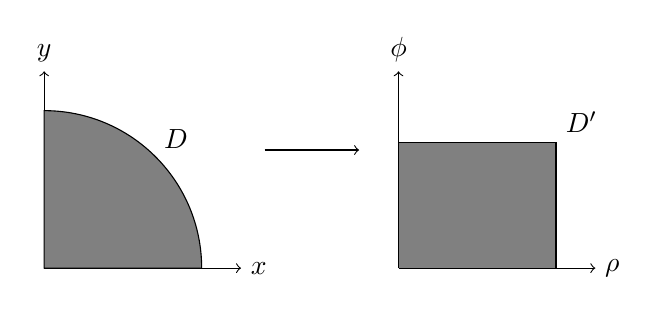
\begin{tikzpicture}
          \draw [->] (0, 0) -- (2.5, 0) node [right] {$x$};
          \draw [->] (0, 0) -- (0, 2.5) node [above] {$y$};
          \draw [fill=gray] (0, 0) -- (2, 0) arc (0:90:2) -- cycle;
          \node at (1.4, 1.4) [anchor=south west] {$D$};
          \draw [->] (2.8,1.5) -- (4,1.5);
          \fill[gray] (4.5,0) rectangle (6.5,1.6);
          \draw [->] (4.5, 0) -- (7, 0) node [right] {$\rho$};
          \draw [->] (4.5, 0) -- (4.5, 2.5) node [above] {$\phi$};
          \draw (4.5,1.6) -- (6.5,1.6) -- (6.5,0);
          \node [above right] at (6.5,1.6) {$ D' $};
        \end{tikzpicture}
      \end{center}
      Hence $ \dd x\dd y=\rho\dd \rho\dd \phi $
      \[
          \iint_{D}f(x,y)\dd x\dd y = \iint_{D'}f(\rho \cos \phi,\rho \sin \phi)\rho \dd \rho\dd \phi.
      \]
      Take $ R\to \infty $,
      \[
          \int_{x=0}^{\infty} \int_{y=0}^{\infty} f(x,y) \,\mathrm{d}y \,\mathrm{d}x = \int_{\phi=0}^{\pi/2} \int_{\rho=0}^{\infty} f(\rho \cos \phi,\rho \sin \phi) \rho \,\mathrm{d}\rho \,\mathrm{d}\phi.
      \]

      Now consider 
      \[
          I = \int_{0}^{\infty} e^{-x^2} \,\mathrm{d}x.
      \]
      Have 
      \begin{align*}
          I^2 &= \int_{0}^{\infty} e^{-x^2} \,\mathrm{d}x \cdot \int_{0}^{\infty} e^{-y^2} \,\mathrm{d}y \\ 
          &= \int_{x=0}^{\infty} \int_{y=0}^{\infty} e^{-(x^2+y^2)} \,\mathrm{d}y \,\mathrm{d}x\\ 
          &= \int_{\phi=0}^{\pi/2} \int_{\rho=0}^{\infty} e^{-\rho^2} \rho \,\mathrm{d}\rho \,\mathrm{d}\phi \\
          &= \frac{\pi}{2} \int_{0}^{\infty} \frac{\mathrm{d}}{\mathrm{d}\rho}\left( -\frac{1}{2}e^{-\rho^2} \right)  \,\mathrm{d}\rho = \frac{\pi}{4}.
      \end{align*}
      Hence $ I=\sqrt{\pi}/2 $.
\end{example}